\documentclass{article}
\usepackage[a4paper]{geometry}
\usepackage[utf8]{inputenc}
\usepackage{amsmath}
\usepackage{amssymb}
\usepackage{tikz}
\usetikzlibrary{automata,positioning}

\title{Modelos de Computacion - Practicas}
\date{27-11-2017}
\author{Eloy Bedia Garcia}
\geometry{top=2cm, bottom=2cm, left=2cm, right=1cm}

\begin{document}
  \pagenumbering{gobble}
  \maketitle

  \newpage
  \pagenumbering{roman}

\section{Práctica 1}

\hspace{0,5cm}	1. Dada la gramatica G = (\{S,A\} , \{a,b\}, P, S) donde P =  $\{S  \rightarrow  abAS, abA  \rightarrow  baab, S  \rightarrow  a, A  \rightarrow  b \}$.

Determinar el lenguaje que genera:\\

\hspace{1cm}  $L = \{u a \mid u \in  \{baab,abb\}^+\}$ \\

\vspace{0,65cm}

2. Sea la gramatica G = (V,T,P,S) donde:

\hspace{1cm}	$V = \{<numero>,<digito>\}$

\hspace{1cm}	$T = \{0,1,2,3,4,5,6,7,8,9\}$

\hspace{1cm}	$S = <numero>$\\

\hspace{1cm}	Las reglas de produccion P son las siguientes:
	
\hspace{2cm}	$<numero> \rightarrow <digito><numero>$

\hspace{2cm}	$<numero> \rightarrow <digito>$

\hspace{2cm}	$<digito> \rightarrow 0\mid 1 \mid 2 \mid 3 \mid 4 \mid 5 \mid 6 \mid 7 \mid 8 \mid 9$\\

Determinar el lenguage que genera:\\

 \hspace{1cm}L = $\{ 0,1,2,3,4,5,6,7,8,9 \}^{+}$\\

\vspace{0,65cm}

3. Encontrar si es posible una gramatica libre de contexto que genera el lenguaje L, siendo $L\subseteq\{a,b,c\}^{*}$. La palabra $u \in L \Longleftrightarrow$ o contiene el mismo numero de símbolos b que de símbolos c.\\

  \hspace{1cm}Sea la gramatica G = (V,T,P,S) donde:

  \hspace{2cm}	$V = \{S,A\}$

  \hspace{2cm}	$T = \{a,b,c\}$

  \hspace{2cm}	$S = S$\\

  \hspace{2cm}	Las reglas de produccion P son las siguientes:
	
  \hspace{3cm}	$<numero> \rightarrow bSc \mid A$

  \hspace{3cm}	$<numero> \rightarrow Aa \mid \epsilon$

  \vspace{0,65cm}

4. Encontrar gramaticas de tipo 2 para $L\subseteq\{0,1\}^{*}$. En cada caso, indicar si los lenguajes generados son regulares indicando, si existe una gramatica regular que los genera. Para los siguientes casos:\\
  
\hspace{1cm}a. Palabras que comienzan con 000 y terminan en 111.\\

\hspace{2cm}$G = (\{S,A\},\{0,1\},P,S)$ donde P son las producciones siguientes:\\

\hspace{2cm}$S \rightarrow 000A111$

\hspace{2cm}$A \rightarrow 0A \mid 1A \mid \epsilon$\\

\hspace{2cm} Gramática regular $G = (\{S,A,B\},\{0,1\},P,S)$ donde P son las producciones siguientes:\\

\hspace{2cm}$S \rightarrow 000A$

\hspace{2cm}$A \rightarrow 0A \mid B \mid 111$

\hspace{2cm}$A \rightarrow 1B \mid A \mid 11$\\

 \hspace{1cm}b. Palabras que no contienen dos 0 seguidos (00).\\

\hspace{2cm}$G = (\{S,A\},\{0,1\},P,S)$ donde P son las producciones siguientes:\\
	
\hspace{2cm}$S \rightarrow 0A \mid 1S \mid \epsilon$

\hspace{2cm}$A \rightarrow 1S \mid \epsilon$\\

\hspace{2cm}Este lenguaje es regular, es decir, puede ser generado por una gramatica regular (tipo 3)\\

\hspace{1cm}c. Palabras que si contienen tres ceros (000) le sigue al menos un 1.\\

\hspace{2cm}	$G = (\{S,A,B,C\},\{0,1\},P,S)$ donde P son las producciones siguientes:\\

\hspace{2cm}	$S \rightarrow 0A \mid C \mid \epsilon$
	
\hspace{2cm}	$A \rightarrow 0B \mid C \mid \epsilon$

\hspace{2cm}	$B \rightarrow 0C \mid C \mid \epsilon$

\hspace{2cm}	$C \rightarrow 1S$\\

\hspace{2cm}	Este lenguaje es regular, es decir, puede ser generado por una gramatica regular (tipo 3)\\

\vspace{0,65cm}

5. En una empresa de videojuegos “Dungeons of the Hell” están planteando diseñar una gramatica capaz de generar niveles de un juego de exploracion de mazmorras, y sus salas correspondientes, siguiendo el siguiente conjunto de restricciones:\\

\hspace{1cm}- Hay 2 tipos de salas, grandes (g) y pequeñas (p).\\

\hspace{1cm}- Hay 2 tipos de monstruos, fuertes (f) y débiles (d).\\

\hspace{1cm}- Las salas grandes, contienen al menos 1 monstruo fuerte y 2 debiles. Y las salas pequeñas, contienen a lo sumo 1 monstruo fuerte.\\

\hspace{1cm}- Existen unas salas especiales donde se pueden reponer fuerzas y comprar armas. Estas salas son las llamas salas de tendero (t).\\

\hspace{1cm}- Siempre, tras la sala grande, se va a encontrar una sala secreta (s). Al final de cada nivel habra una sala final donde hay que rescatar a una princesa (x).\\

Elaborar una gramatica que genere estos niveles con sus restricciones. Cada palabra del lenguaje es un solo nivel. ¿A que tipo de gramatica dentro de la jerarquia de Chomsky pertenece la gramatica diseñada? ¿Seria posible diseñar una gramática de tipo 3 para dicho problema?\\

\hspace{1cm}	$G = (\{S,G,P,M\},\{g,p,f,d,t,x\},P,S)$ donde P son las producciones siguientes:\\

\hspace{1cm}	$S \rightarrow GS \mid PS \mid tS \mid x$

\hspace{1cm}	$M \rightarrow fM \mid dM \mid \epsilon$

\hspace{1cm}	$G \rightarrow gMfMdMdM \mid gMdMfMdM \mid gMdMdMf$

\hspace{1cm}	$P \rightarrow pMdM$\\

\hspace{1cm}	Esta gramatica, según la Jerarquía de Chomsky, es de Tipo 2 (Independiente del contexto).

\hspace{1cm}	No existe una gramatica regular que satisfaga estas restricciones, ya que hay que comprobar que exista un mínimo de mosntruos determinados, y para ello es necesaría una gramática de tipo 2
\newpage

\section{Práctica 2}
Dada la URL de un video de Youtube, el software te facilita los siguientes datos:
\hspace{1cm} -Título

\hspace{1cm} -Autor

\hspace{1cm} -ID

\hspace{1cm} -Miniatura

\hspace{1cm} -Nº Likes

\hspace{1cm} -Nº Dislikes

\hspace{1cm} -Nº Visitas

\hspace{1cm} -Duración (s)

\hspace{1cm} -¿Apt para niños?

\begin{figure}[!hp]
\includegraphics[width=\textwidth]{Captura de pantalla de 2018-01-07 17-46-40.jpg}
\centering
\end{figure}

\begin{figure}[!hp]
\includegraphics[width=\textwidth]{Captura de pantalla de 2018-01-07 17-46-55.jpg}
\centering
\end{figure}

\begin{figure}[!hp]
\includegraphics[width=\textwidth]{Captura de pantalla de 2018-01-07 17-47-06.jpg}
\centering 
\end{figure}

\begin{figure}[!hp]
\includegraphics[width=\textwidth]{Captura de pantalla de 2018-01-07 17-47-23.jpg} 
\centering
\end{figure}

\begin{figure}[!hp]
\includegraphics[width=\textwidth]{Captura de pantalla de 2018-01-07 17-47-31.jpg} 
\centering
\end{figure}

\begin{figure}[!hp]
\includegraphics[width=\textwidth]{Captura de pantalla de 2018-01-07 17-47-43.jpg} 
\centering
\end{figure}

\begin{figure}[!hp]
\includegraphics[width=\textwidth]{Captura de pantalla de 2018-01-07 17-47-58.jpg} 
\centering
\end{figure}

\newpage
\section{Práctica 3}

\hspace{0,5cm} 1. Construir un AFD que acepte cada uno de los siguientes lenguajes con alfabeto {0,1}:\\

\hspace{1cm} a. El lenguaje de las palabras que contienen la subcadena 010.\\

\begin{center}
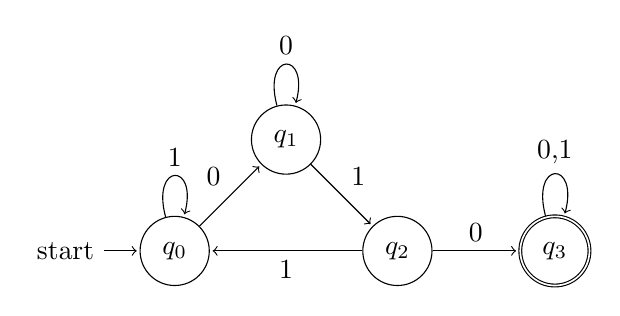
\begin{tikzpicture}[shorten >=1pt,node distance=2cm,on grid,auto]
	\node[state,initial] (q_0) {$q_0$};
	\node[state] (q_1) [above right=of q_0] {$q_1$}; 
	\node[state] (q_2) [below right=of q_1] {$q_2$};
	\node[state,accepting] (q_3) [right=of q_2] {$q_3$};

	\path[->]
	(q_0) edge node {0} (q_1)
	      edge [loop above] node {1} ()

	(q_1) edge [loop above] node {0} ()
	      edge node {1} (q_2)

	(q_2) edge node {0} (q_3)
	      edge node {1} (q_0)

	(q_3) edge [loop above] node {0,1} ();
\end{tikzpicture}
\end{center}

\hspace{1cm} b. El lenguaje de las palabras que empiezan o terminan (o ambas cosas) en 010.\\

\begin{center}
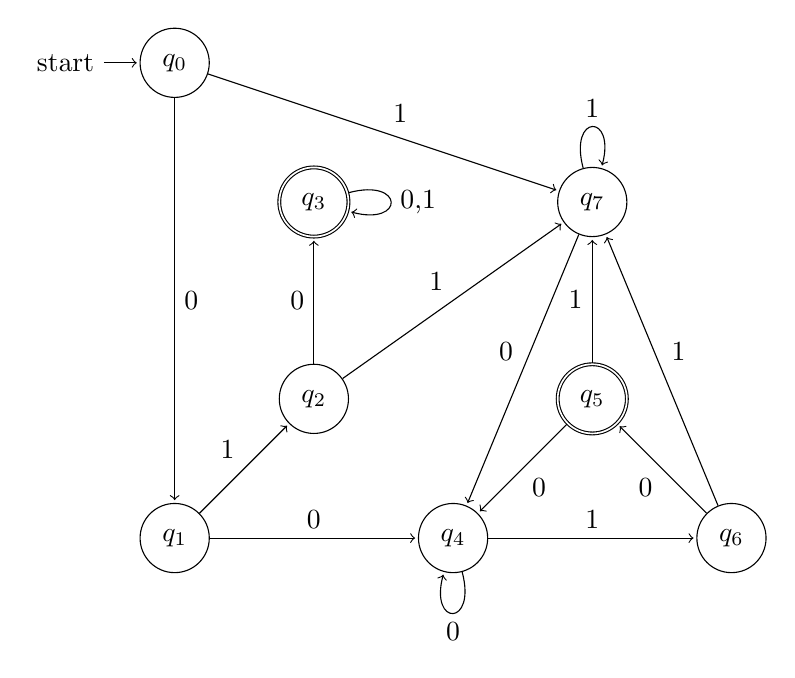
\begin{tikzpicture}[shorten >=1pt,node distance=2.5cm,on grid,auto]
	\node[state] (q_1) {$q_1$}; 
	\node[state] (q_2) [above right=of q_1] {$q_2$};
	\node[state,accepting] (q_3) [above=of q_2]{$q_3$};
	\node[state,initial] (q_0) [above left=of q_3] {$q_0$};
	\node[state] (q_4) [below right=of q_2] {$q_4$};
	\node[state,accepting] (q_5) [above right=of q_4] {$q_5$};
	\node[state] (q_6) [below right=of q_5] {$q_6$};
	\node[state] (q_7) [above=of q_5] {$q_7$};

	\path[->]
	(q_0) edge node {0} (q_1)
	      edge node {1} (q_7)

	(q_1) edge node {0} (q_4)
	      edge node {1} (q_2)

	(q_2) edge node {0} (q_3)
	      edge node {1} (q_7)

	(q_3) edge [loop right] node {0,1} ()

	(q_4) edge [loop below] node {0} ()
	      edge node {1} (q_6)

	(q_5) edge node {0} (q_4)
	      edge node {1} (q_7)

	(q_6) edge node {0} (q_5)
	      edge node [swap] {1} (q_7)

	(q_7) edge node [swap] {0} (q_4)
	      edge [loop above] node {1} ();

\end{tikzpicture}
\end{center}

\hspace{1cm} c. El lenguaje $L \subset \{0, 1\}^{*}$ de todas las palabras con un número impar de ocurrencias de\\
\hspace{1cm} la subcadena 01.

\begin{center}
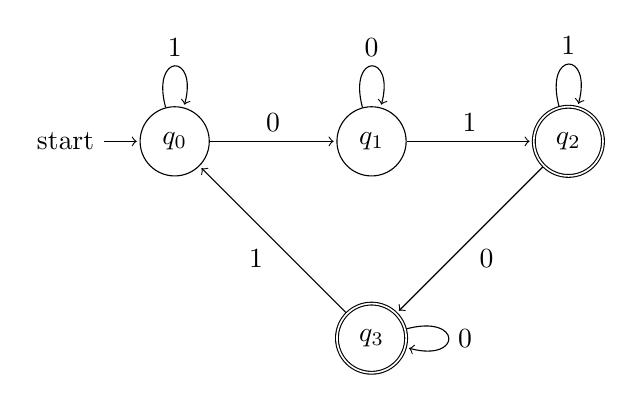
\begin{tikzpicture}[shorten >=1pt,node distance=2.5cm,on grid,auto]
	\node[state,initial] (q_0) {$q_0$};
	\node[state] (q_1) [right=of q_0] {$q_1$}; 
	\node[state,accepting] (q_2) [right=of q_1] {$q_2$};
	\node[state,accepting] (q_3) [below=of q_1]{$q_3$};

	\path[->]
	(q_0) edge node {0} (q_1)
	      edge [loop above] node {1} ()

	(q_1) edge [loop above] node {0} ()
	      edge node {1} (q_2)

	(q_2) edge node {0} (q_3)
	      edge [loop above] node {1} ()

	(q_3) edge [loop right] node {0} ()
	      edge node {1} (q_0);


\end{tikzpicture}
\end{center}

\vspace{0,65cm}

2. Construir un AFND que acepte cada uno de los siguientes lenguajes con alfabeto {0,1}:


\hspace{1cm} a. El lenguaje de las palabras que terminan en 010.\\
\begin{center}
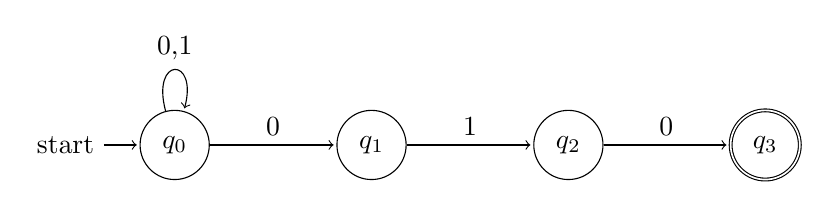
\begin{tikzpicture}[shorten >=1pt,node distance=2.5cm,on grid,auto]
	\node[state,initial] (q_0) {$q_0$};
	\node[state] (q_1) [right=of q_0] {$q_1$}; 
	\node[state] (q_2) [right=of q_1] {$q_2$};
	\node[state,accepting] (q_3) [right=of q_2]{$q_3$};

	\path[->]
	(q_0) edge [loop above] node {0,1} ()
	      edge node {0} (q_1)

	(q_1) edge node {1} (q_2)

	(q_2) edge node {0} (q_3);

\end{tikzpicture}
\end{center}

\hspace{1cm} b. El lenguaje de las palabras que empiezan o terminan (o ambas cosas) en 010.\\

\begin{center}
\begin{tikzpicture}[shorten >=1pt,node distance=2.5cm,on grid,auto]
	\node[state,initial] (q_0) {$q_0$};
	\node[state] (q_1) [above right=of q_0] {$q_1$}; 
	\node[state] (q_2) [right=of q_1]{$q_2$};
	\node[state] (q_3) [right=of q_2] {$q_3$};
	\node[state,accepting] (q_4) [right=of q_3] {$q_4$};
	\node[state] (q_5) [below right=of q_0] {$q_5$};
	\node[state] (q_6) [right=of q_5]{$q_6$};
	\node[state] (q_7) [right=of q_6] {$q_7$};
	\node[state,accepting] (q_8) [right=of q_7] {$q_8$};

	\path[->]

	(q_0) edge node {$\epsilon$} (q_1)
	      edge node {$\epsilon$} (q_5)
	

	(q_1) edge node {0} (q_2)

	(q_2) edge node {1} (q_3)

	(q_3) edge node {0} (q_4)

	(q_4) edge [loop above] node {0,1} ()
	     

	(q_5) edge [loop below] node {0,1} ()
	      edge node {0} (q_6)

	(q_6) edge node {1} (q_7)

	(q_7) edge node {0} (q_8);

\end{tikzpicture}
\end{center}


3. Diseñar una Máquina de Mealy o de Moore que, dada una cadena usando el alfabeto A={‘a’,‘w’, ‘o’} encienda un led verde (salida ‘V’) cada vez que se detecte la cadena “woow” en la entrada apagándolo cuando lea cualquier otro símbolo después de esta cadena (representamos el led apagado con la salida“X“). El autómata tiene que encender el led verde (salida ‘V’) , tantas veces como aparezca en la secuencia “woow” en la entrada, y esta secuencia puede estar solapada. Por ejemplo ante la siguiente entrada, la Máquina de Mealy/Moore emitirá la salida:  

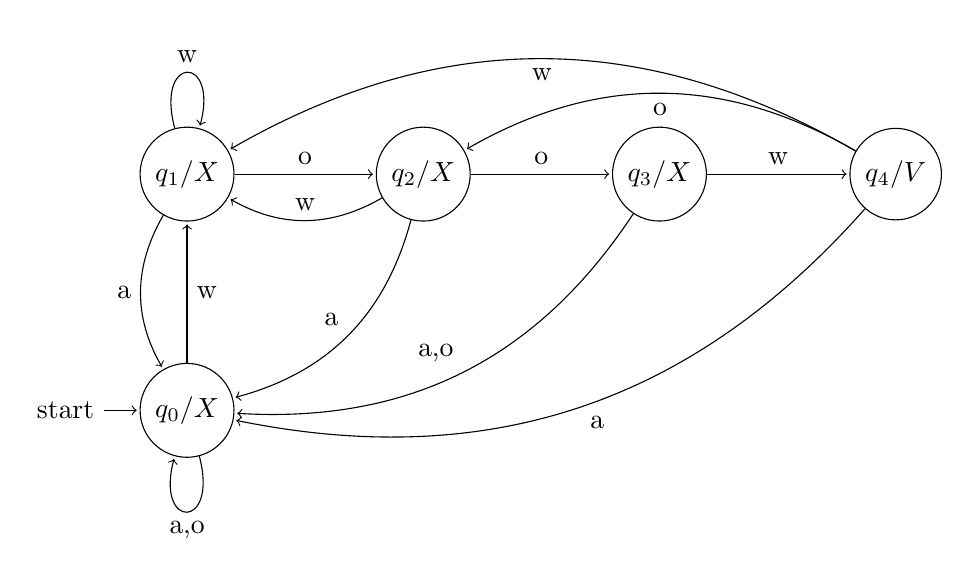
\begin{tikzpicture}[shorten >=1pt,node distance=3cm,on grid,auto]
	\node[state] (q_1X) {$q_1/X$};
	\node[state,initial] [below=of q_1X] (q_0X) {$q_0/X$};
	\node[state] (q_2X) [right=of q_1X] {$q_2/X$};
	\node[state] (q_3X) [right=of q_2X] {$q_3/X$};
	\node[state] (q_4V) [right=of q_3X] {$q_4/V$};

	\path[->]

	(q_0X) edge [loop below] node {a,o} ()
	      edge node [swap] {w} (q_1X)

	(q_1X) edge [bend right] node [swap] {a} (q_0X)
	       edge [loop above] node {w} ()
	       edge node {o} (q_2X)

	(q_2X) edge [bend left] node [swap] {a} (q_0X)
	       edge [bend left] node [swap] {w} (q_1X)
	       edge node {o} (q_3X)

	(q_3X) edge [bend left] node [swap] {a,o} (q_0X)
	      edge node {w} (q_4V)

	(q_4V) edge [bend right] node {w} (q_1X)
	      edge [bend right] node {o} (q_2X)
	      edge [bend left] node {a} (q_0X);
\end{tikzpicture}

\vspace{0,65cm}

4. Obtener un AFD equivalente al AFND siguiente:

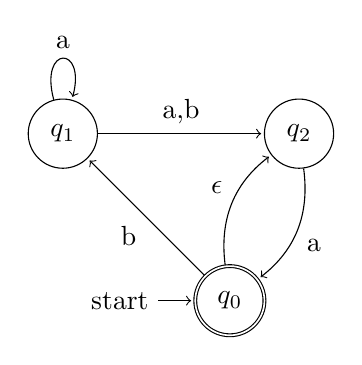
\begin{tikzpicture}[shorten >=1pt,node distance=3cm,on grid,auto]
	\node[state] (q_1) {$q_1$};
	\node[state,initial,accepting] [below right=of q_1] (q_0) {$q_0$};
	\node[state] (q_2) [right=of q_1] {$q_2$};


	\path[->]

	(q_0) edge node {b} (q_1)
	      edge [bend left] node {$\epsilon$} (q_2)

	(q_1) edge [loop above] node {a} ()
	      edge node {a,b} (q_2)

	(q_2) edge [bend left] node {a} (q_0);

\end{tikzpicture}


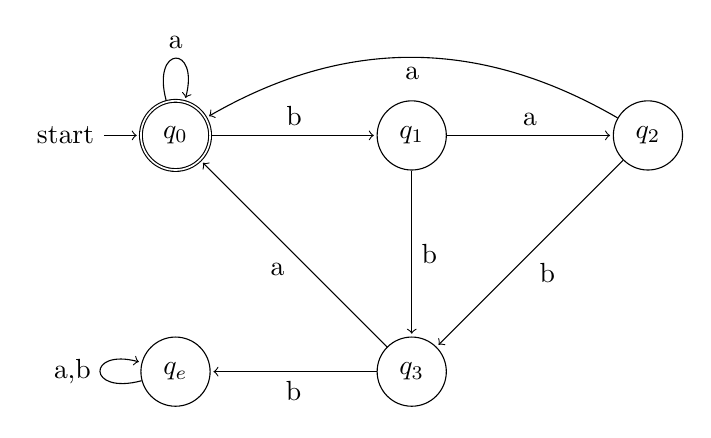
\begin{tikzpicture}[shorten >=1pt,node distance=3cm,on grid,auto]
	\node[state,initial,accepting] (q_0) {$q_0$};
	\node[state] (q_1) [right=of q_0] {$q_1$};
	\node[state] (q_2) [right=of q_1] {$q_2$};
	\node[state] (q_3) [below=of q_1] {$q_3$};
	\node[state] (q_e) [below=of q_0] {$q_e$};


	\path[->]

	(q_0) edge [loop above] node {a} ()
	      edge node {b} (q_1)

	(q_1) edge node {a} (q_2)
	      edge node {b} (q_3)

	(q_2) edge [bend right] node {a} (q_0)
	      edge node {b} (q_3)

	(q_3) edge node {a} (q_0)
	      edge node {b} (q_e)

	(q_e) edge [loop left] node {a,b} ();

\end{tikzpicture}

\newpage

\section{Práctica 4}

1. Determinar cuáles de las siguientes gramáticas son ambiguas y, en su caso, comprobar si los lenguajes generados son inherentemente ambiguis. Justificar la resuesta: \\

\hspace{1cm} a. $S \rightarrow AbB$ $A \rightarrow aA \mid \epsilon$ $B \rightarrow aB \mid bB \mid \epsilon$ 

\hspace{1cm} No es ambigua, ya que produce a's al principio; y a's y b's al final.

\hspace{1cm} b. $S \rightarrow abaS \mid baS \mid babS \mid \epsilon$ 

\hspace{1cm} Es ambigua, ya haciendo 3 veces la producción 2 se puede llegar al mismo resultado que haciendo una vez la 3 y la 1.

\hspace{1cm} El lenguaje no es inherente mente ambiguo, ya que la siguiente gramatica no ambigua genera el mismo leguaje:

\hspace{2cm} $S \rightarrow aA \mid bC \mid \epsilon$

\hspace{2cm} $A \rightarrow bB$

\hspace{2cm} $B \rightarrow aS$

\hspace{2cm} $C \rightarrow aD$

\hspace{2cm} $C \rightarrow bS \mid aA \mid \epsilon$\\

\hspace{1cm} c. $S \rightarrow aSA \mid \epsilon$ $A \rightarrow bA \mid \epsilon$ 

\hspace{1cm} Es ambigua, ya que produciendo N a's puedo producir hasta N b's, con lo que llevando a vacio cualquier A $\le$ N b's puedo obtener una palabra con N a's y N - A b's.

\vspace{0,65cm}

2. Encontrar el autómata con pila que acepte el siguiente lenguaje L.\\

\begin{center}
$L = {x^{i}y^{j}z^{k} \mid i+k=j; i,j,k \in N}$
\end{center}

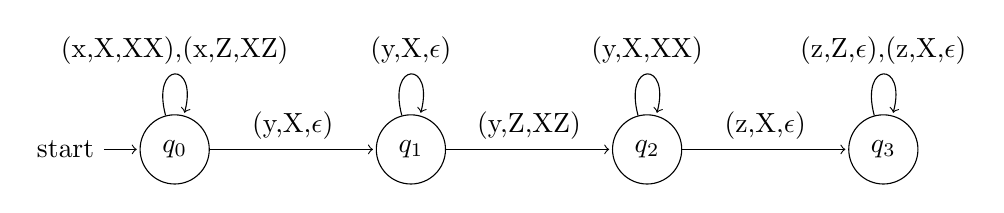
\begin{tikzpicture}[shorten >=1pt,node distance=3cm,on grid,auto]
	\node[state,initial] (q_0) {$q_0$};
	\node[state] (q_1) [right=of q_0] {$q_1$};
	\node[state] (q_2) [right=of q_1] {$q_2$};
	\node[state] (q_3) [right=of q_2] {$q_3$};

	\path[->]

	(q_0) edge [loop above] node {(x,X,XX),(x,Z,XZ)} ()
	      edge node {(y,X,$\epsilon$)} (q_1)

	(q_1) edge [loop above] node {(y,X,$\epsilon$)} ()
	      edge node {(y,Z,XZ)} (q_2)

	(q_2) edge [loop above] node {(y,X,XX)} ()
	      edge node {(z,X,$\epsilon$)} (q_3)

	(q_3) edge [loop above] node {(z,Z,$\epsilon$),(z,X,$\epsilon$)} ();

\end{tikzpicture}

\hspace{1cm} Gramática:

\hspace{2cm} $S \rightarrow aSb \mid bSa$

\vspace{0,65cm}

3. Pasar  este  autómata  con  pila  a  gramática  independiente  del  contexto.  Una  vez conseguida  la  gramática, proceder a  eliminar  variables  y  producciones inútiles.  ¿Qué lenguaje genera dicha gramática? 

\hspace{1cm} $S \rightarrow aAS \mid \epsilon$

\hspace{1cm} $A \rightarrow aAA \mid b$

El lenguaje generado por esta gramatica  pertenece a $\{a,b\}^{*}$ tal que para toda a perteneciente a $\{a,b\}^{*}$ si la divides por la mitad tiene el mismo número de a's que de b's

\vspace{0,65cm}

4. Dar gramáticas libres de contexto o regulares no ambiguas (cuando sea posible) para los siguientes lenguajes: 

\hspace{1cm} a. $L_{1} = {(ab)^{i}(bc)^{j} \mid i,j \ge  0}$

\hspace{2cm} 	$S \rightarrow abS \mid B$

\hspace{2cm} 	$B \rightarrow bcB \mid \epsilon$\\

\hspace{1cm} b. $L_{2} = {a^{i}b^{j}c^{i+j} \mid i,j \ge  0}$

\hspace{2cm} 	$S \rightarrow aSc \mid A$

\hspace{2cm} 	$A \rightarrow bAc \mid \epsilon$\\

\hspace{1cm} c. $L_{3} = {a^{i}b^{j}c^{j}d^{i} \mid i,j \ge  0}$

\hspace{2cm} 	$S \rightarrow aSd \mid A$

\hspace{2cm} 	$A \rightarrow bAc \mid \epsilon$

\hspace{1cm} d. $L_{4}$ definido como el conjunto de palabras de alfabeto {a, b, c} que empiezan por aab y acaban por bbc y tales que estas dos subcadenas no aparecen nunca en el interior de la palabra (sólo al comienzo y al final).

\hspace{2cm} 	$S \rightarrow aabAbbc$

\hspace{2cm} 	$A \rightarrow aA_{1} \mid bA_{3} \mid cA$

\hspace{2cm} 	$A_{1} \rightarrow aA_{2} \mid bA_{3} \mid cA$

\hspace{2cm} 	$A_{2} \rightarrow aA_{2} \mid cA$

\hspace{2cm} 	$A_{3} \rightarrow bA_{4} \mid aA_{1} \mid cA$

\hspace{2cm} 	$A_{4} \rightarrow aA_{1} \mid bA_{4}$

\end{document}
